% !TEX root = ../main.tex
\section{Návrh implementácie riadenia}
\label{sec:technologies}

Našou úlohou v~tejto bakalárskej práci je naprogramovať a~otestovať nami vytvorený ovládač pre~mobilného
robota. Na~vyber máme viacero technológii, ktoré môžeme použiť. Na~vytvorenie ovládača budeme potrebovať
operačný systém na~počítači, ktorý budeme použivať na~programovanie a~testovanie. Na~výber máme dve možnosti.
Menovite to~sú~operačný systém \textit{Windows} alebo operačný systém \textit{Ubuntu}, ktorý je založený
na~jadre Linux. Ďalšiu vec, ktorú budeme potrebovať je programovací jazyk. Na~výber máme z~veľmi veľa
možností a~to~hlavne \textit{C}, \textit{C++}, \textit{Python}, \textit{Java} alebo \textit{Matlab}.
Keďže, zo~zadania vypláva, že~máme použiť Robotický operačný systém, tak~máme na~výber dve možnosti.
Sú~to~Robotický operačný systém prvej verzie (\textit{ROS1}) a~Robotický operačný systém druhej verzie
(\textit{ROS2}). Na~vytvorenie ovládača môžeme využiť aj~už~naprogramované baličky. Jednou z~možností
je \textit{ros\_control} pre~Robotický operačný systém prvej verzie a~\textit{ros2\_control} pre~Robotický
operačný systém druhej verzie. Samozrejme na~implementáciu a~otestovanie potrebujeme samotného robota.
Pred tým ako začneme preberať spomenutý ovládač a~robota, ktorého budeme riadiť, tak~si predstavíme
technológie, ktoré budeme používať pri~vytváraní ovládača.

\subsection{Operačný systém}
\label{sec:operating_system}

Na~začiatku našej práce sme sa museli rozhodnúť, či~budeme písať program na~náš ovládač v~operačnom systéme Windows 11 alebo
v~operačnom systéme Ubuntu, ktorý je založený na~jadre Linux. Ako programátori sme už~dlhšie pracovali s~operačným systémom
Ubuntu a~poznáme aj~jeho výhody, aj~nevýhody. To~isté platí aj~pre~operačný systém Windows. Toto sú~fakty, ktoré sme zvažovali
pri~výbere operačného systému, ktorý sme používali počas celej bakalárskej práce.

\subsubsection{Windows}
\label{sec:windows}

Windows je najpoužívanejším operačným systémom na~počítače na~svete. Je to~hlavne preto, že~je jednoduchý na~používanie
pre~netechnicky založených užívateľov. Windows ale~nie je bezpečným operačným systémom a~taktiež aj~jeho stabilita a~rýchlosť
nie sú~na~najvyššej úrovni. Tento operačný systém používajú lúdia hlavne na~voľnočasové aktivity ako je hranie hier
alebo v~práci ako napríklad v~kanceláriách na~úpravu tabuliek. Pre~nás ako programátorov tento operačný systém nie je
výhodný. Nastavovanie prostredia pre~programovanie je v~tomto operačnom systéme oveľa náročnejšie ako v~operačnom systéme
s~Linuxovým jadrom. Podpora prekladačov programov (z~anglického compiler) je v~tomto operačnom systéme oveľa horšia
ako už~v~spomenutom Linuxe.

\subsubsection{Ubuntu}
\label{sec:ubuntu}

Ubuntu je stabilný a~bezpečný operačný systém, ktorý je založený na~Linuxe. Väčšina ľudí hovorí o~Linuxe ako o~operačnom systéme. Pravdou
to~ale~nie je. Linux je totižto len \textbf{kernel} (jadro) operačného systému. Kernel je hlavný program, ktorý sa stará o~správu hardvéru,
riadenie procesov a~správu pamäte. Zároveň poskytuje možnosť operačnému systému komunikovať s~hardvérom a~poskytuje jednotlivým programom
prístup k~hardvéru a~jeho častiam~\cite{chatgpt}.

Linux je používaný skoro vo~všetkých mobilných zariadeniach, serveroch, cloudoch (dátové servery, na~ktoré sa pripájame cez~internet)
a~ďalších elektronických zariadeniach, ktoré potrebujú rýchlosť, stabilitu a~bezpečnosť. Je taktiež používaný vo~všetkých mobilných
robotoch. Nad~operačným systémom Windows má niekoľko výhod.

\begin{itemize}
	\item \textbf{Open source} Linux je open source jadro pre~operačný systém, čo znamená, že~kód,\\
		ktorý tvorí jeho základ, je k~dispozícii pre~všetkých zadarmo a~každý môže prispieť
		k~jeho vylepšeniu. Tento otvorený prístup umožňuje programátorom prispôsobiť si Linux
		pre~svoje potreby a~vytvárať programy, ktoré sú~optimálne pre~ich prácu. Na~Linuxe
		sú~založené aj~operačné systémy reálneho času alebo software pre~smart mobilné telefóny
		ako je napríklad operačný systém Android.

	\item \textbf{Programovacie nástroje} Linux obsahuje mnoho vynikajúcich programovacích nástrojov, ktoré sú~k~dispozícii
		zadarmo a~sú~široko používané programátormi. Napríklad k~dispozícii v~Linuxe sú~(GCC) \acrlong{GCC} (Kolekcia GNU prekladačov)
		(GNU je skratka pre~\acrlong{GNU}) a~GNU Debugger (GDB) sú~vynikajúce nástroje pre~C/C++ programátorov.

	\item \textbf{Bezpečnosť} Linux má reputáciu bezpečnejšieho operačného systému v~porovnaní s~operačným systémom Windows.
		V~Linuxe je ťažšie infikovať sa škodlivými programami ako je~vírus alebo malware, pretože programy majú obmedzené
		oprávnenie a~prístup k~ďalším súborom. Systém je navrhnutý tak, aby bol odolný voči útokom.

	\item \textbf{Stabilita} Linux má tendenciu byť stabilnejší než Windows, pretože nie je závislý na~ovládačoch a~softvéri
		od~tretích strán. Linux poskytuje jednotný prístup k~správe a~aktualizácii softvéru. Pri~vylepšovaní systému nie je
		za~potreby reštartovať počítač alebo server čo má za~dôsledok zvýšenie spoľahlivosti zariadenia.

	\item \textbf{Flexibilita} Linux je veľmi flexibilný operačný systém, ktorý umožňuje programátorom prispôsobiť si svoje pracovné
		prostredie a~používať programy, ktoré najlepšie vyhovujú ich potrebám. Linux dovoľuje upraviť samotné jadro
		operačného systému a~vybrať si z~neho len tie časti, ktoré užívateľ potrebuje. Tie, ktoré nepotrebuje sa
		v~systéme nenachádzajú. Týmto spôsobom sa zvyšuje rýchlosť systému a~zabezpečuje sa jeho bezpečnosť.

	\item \textbf{Podpora a~komunita} Linux má veľkú a~aktívnu komunitu. Ta obsahuje ako aj~programatorov tak~aj
		netechnicky založených ľudí. Táto komunita poskytuje podporu a~rieši problémy. Vďaka tomu, že~Linux je
		open source, mnoho ľudí prispieva k~jeho vylepšeniu a~vytvára nové programy, čo znamená, že~je vždy
		niečo nové na~objavovanie.

	\item \textbf{Komplexnosť} Napriek všetkým týmto výhodám má Linux aj~svoje nevýhody. Najväčšou nevýhodou, ktorú je treba
		spomenúť je komplexnosť operačného systému. Linux je komplexnejší ako operačný systém Windows, hlavne kvôli svojej
		flexibilnosti. Tým, že~si vieme nastaviť vlastné prostredie, typ systému správy súborov, programy na~sťahovanie,
		publikovanie a~správy balíčkov. Ľudia, ktorí nevedia tento systém opraviť, často siahajú po~preinštalovaní
		systému.
\end{itemize}

\noindent Vďaka svojim výhodám sme sa rozhodli použiť operačný systém Ubuntu verzie 22.04.

\subsection{Programovací jazyk a~jeho prostredie}
\label{sec:programovaci_jazyk}

Medzi programovacie jazy, ktoré by sme mohli použiť patria: \textit{C++}, \textit{C}, \textit{Python},
\textit{Matlab}, \textit{Java}. Aby sme sa rozhodli, ktorý jazyk použijeme pri~vytváraní ovládača, tak~sme si spísali
ich výhody a~nevýhody.

\begin{itemize}
	\item \textbf{C a~C ++}: C a~C ++ sú~hlavné jazyky používané pri~vývoji ROS aplikácií. Sú~to~výkonné a~efektívne jazyky,
		ktoré možno použiť na~nízko úrovňové programovanie, ako sú~riadiace slučky, ovládače a~systémové programovanie.
		C++ je najčastejšie používaný jazyk v~ROS2.

	\item \textbf{Java}: Java je ďalší jazyk, ktorý sa môže použiť na~implementáciu aplikácií v~Robotickom operačnom
		systéme. Je menej bežné používaný ako jazyk C++, ale~má výhodu, a~to~takú, že~je prenositeľný jazyk, ktorý môže
		byť spustený na~akejkoľvek platforme, ktorá podporuje JVM (\acrlong{JVM}) (Virtuálny stroj podporujúci Javu).
		Java je vhodná pre~vývoj vysoko úrovňových komponentov robotického systému, ako sú~GUI (z~anglického \acrlong{GUI})
		(užívateľské rozhranie) a~sieťová komunikácia.

	\item \textbf{Python}: Python je populárny jazyk pre~vývoj ROS2 kvôli svojej čitateľnosti a~jednoduchosti použitia.
		Je vhodný pre~vývoj vysoko úrovňových komponentov robotického systému, ako sú~algoritmy na~rozhodovanie,
		spracovanie dát a~vizualizácia.

	\item \textbf{Matlab}: Matlab je vysoko úrovňový programovací jazyk a~prostredie používané vo~vedeckom prostredí,
		analýze dát a~vizualizácii. Je to~výkonný jazyk pre~numerické výpočty a~často sa používa na~simulovanie
		a~testovanie algoritmov pre~roboty. Avšak, nie je bežne používaný v~ROS2 vývoji. Na~použivanie tohto rozhrania
		je spravený modul \textit{ROS Toolbox}, ktorý zabezpečuje jednoduchú implementáciu uzlov a~ich komunikácie.

	\item \textbf{Výkon}: C a~C++ poskytujú najlepší výkon pre~ROS aplikácie kvôli ich nízkoúrovňovej implementácii a~priamemu
		prístupu k~pamäti. Python, Matlab a~Java sú~pomalšie ako C a~C ++ kvôli ich interpretácii.

	\item \textbf{Čas vývoja}: Python a~Java sa vyvíjajú rýchlejšie ako C a~C++ kvôli ich jednoduchosti a~jednoduchosti
		použitia. Matlab môže byť tiež rýchlejší pri~vývoji pre~určité úlohy vďaka svojim zabudovaným knižniciam a~nástrojom.
		Medzi tieto nástroje patri napríklad \textit{Simunlink} alebo \textit{Stateflow}.

	\item \textbf{Kompatibilita}: Všetky uvedené jazyky môžu byť použité s~Robotickým operačnom systémom a~môžu
		komunikovať s~robotom pomocou TCP/IP komunikácie.
\end{itemize}

Na~základe vyššie spomenutých rozdielov sme sa rozhodli použiť programovací jazyk \textit{C++}. Toto rozhodnutie sme spravili
hlavne kvôli jeho možnostiam v~implementácii tried, výkonu a~podpore v~komunite.

\subsection{Robotický operačný systém}
\label{sec:ros}

Robotický operačný systém (ROS) (\acrlong{ROS}) je súbor voľne dostupných softvérových knižníc a~nástrojov, ktoré vytvárajú
vhodné podmienky pre~programátorov na~písanie aplikácií pre~mnohé druhy robotov. ROS má dve verzie. Vo~všeobecnosti sa stretneme
s~tým, že~pod názvom ROS1 alebo ROS sa myslí ROS verzie 1. Pod názvom ROS2 sa myslí ROS verzie 2. Aby nenastali nejasnosti
budeme v~tomto dokumente označovať ROS verzie 1 ako ROS1 a~ROS verzie 2 ako ROS2. V~prípade, keď budme hovoriť o~spoločných
vlastnostiach a~funkcionalitách, ROS1 a~ROS2 budeme označovať dokopy ako ROS.

ROS je open source, čo znamená, že~ide o~softvér uvoľnený pod licenciou, kde~má používateľ práva na~použitie,
štúdium, zmenu a~redistribúciu. Mnohé open source licencie však určujú určité obmedzenia na~tieto práva pre~tento softvér,
ale~v~podstate môžeme predpokladať tieto práva. Najbežnejšie licencie pre~ROS2 softvérové balíčky sú~Apache 2 a~BSD,
hoci vývojári majú slobodu používať aj~iné \cite{ROS2book}. Využitia Robotického operačného systému v~reálnom svete sa môžu
objaviť v~automobiloch, mobilných robotoch, dronoch alebo manipulátoroch.

\subsubsection{Základné pojmy}
\label{sec:zakladne_pojmy}

Komunikácia v~ROSe je zabezpečená cez~IPC (\acrlong{IPC}), TCP/IP a~UDP/IP komunikáciou pomocou troch zakladacích metód:
\textbf{témy} (Topics), \textbf{služby} (Services) a~\textbf{akcie} (Actions).
Všetky tieto metódy slúžia na~posielanie správ na~synchronizáciu vykonávania programu a~komunikáciu jednotlivých častí programu.
Na~to~aby sme ich vedeli správne využiť musíme poznať ich základnú implementáciu a~funkcionalitu. Správanie týchto metód je nasledovné.

\subsubsection{Témy}
\label{sec:topic}

	\textbf {Témy} sú~sprostredkované pomocou IPC, medzi procesová komunikácia z~anglického \acrlong{IPC},
	alebo TCP/IP komunikácie . Je to~najjednoduchší spôsob komunikácie. Komunikáciu cez~témy si vieme prirovnať k~UDP/IP
	protokolu, s~tým že~nemusia prebiehať cez~sieť. Definujeme si jedného poskytovateľa (publishers) a~jedného
	alebo viacerých príjemcov (subscribers). Medzi týmito dvoma alebo viacerými účastníkmi sa následne
	posielajú správy (messages), ktoré sme si dopredu definovali. Parametre a~obsah týchto správ je
	definovaný priamo v~téme. Nové témy si vieme sami vytvoriť. V~prípade, že~chceme vytvoriť novú tému, musíme
	si vytvoriť nový balíček, v~ktorom si spravíme súbor s~príponou \textit{.msg}.

	\begin{figure}[!htbp]
		\centering
		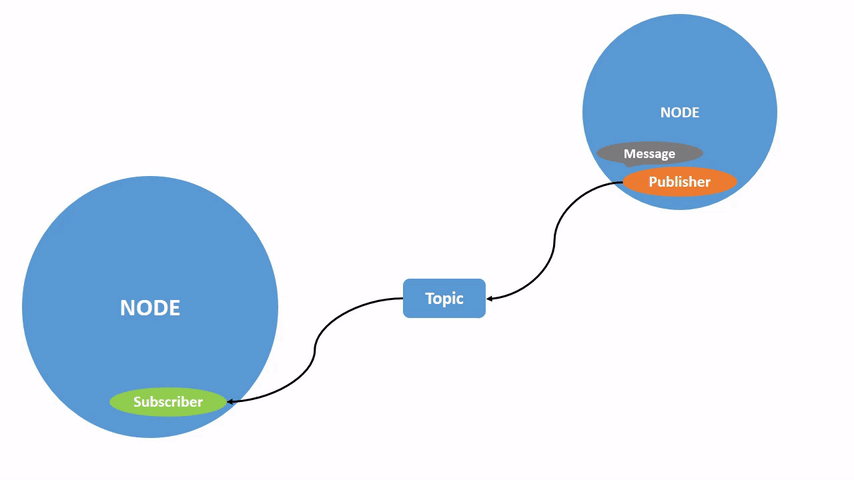
\includegraphics[width=8cm]{img/topicsExplanation.png}
		\caption{Vizualizácia témy v~ROSe~\cite{RosDoc}}
		\label{fig:topics}
	\end{figure}

\clearpage

\subsubsection{Služby}
\label{sec:services}

	\textbf {Služby} sú~sprostredkované pomocou TCP/IP protokolu. Poskytujú nám rovnaký spôsob komunikácie ako témy, až na~to, že~sa správy
	medzi servisom a~klientom posielajú cez~LAN (\acrlong{LAN}). Tieto správy sa posielajú oboma smermi. Služby sa využívajú pri~komunikácii
	medzi viacerými zariadeniami. Jedno zariadenie posiela požiadavku (request) a~druhe zariadenie túto požiadavku prime
	a~spracuje. Po~spracovaní pošle naspäť odpoveď (response). Odpoveď môže obsahovať jednoduchú potvrdenie, alebo inú
	komplexnejšiu štruktúru. Nové služby si vieme sami vytvoriť. V~prípade, že~chceme vytvoriť novú službu, musíme
	si vytvoriť nový balíček, v~ktorom si spravíme súbor s~príponou \textit{.srv}.

	\begin{figure}[!htbp]
		\centering
		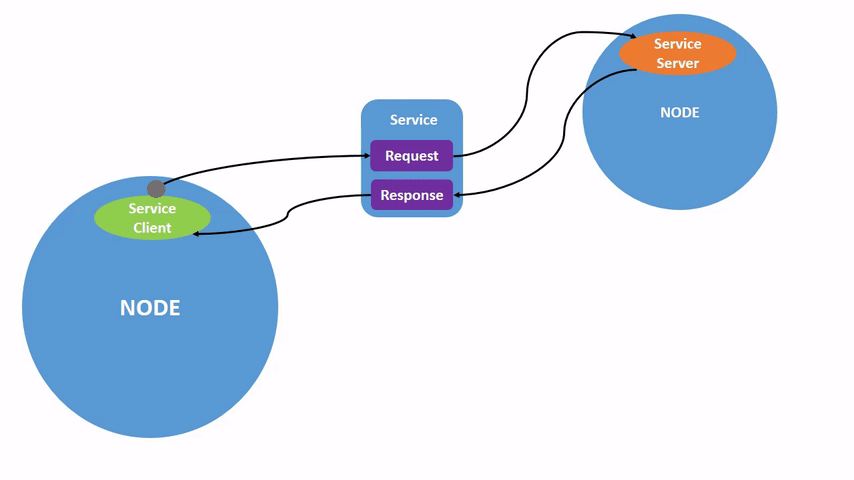
\includegraphics[width=8cm]{img/serviceExplanation.png}
		\caption{Vizualizácia služby v~ROSe~\cite{RosDoc}}
		\label{fig:service}
	\end{figure}

\subsubsection{Akcie}
\label{sec:actions}
	\textbf {Akcie} sú~taktiež sprostredkované TCP/IP protokolom. Sú~najzložitejším spôsobom
	komunikácie. Tento spôsob bol pridaný do~ROS1 až neskôr. V~druhej verzii ROSu je tento
	typ komunikácie medzi troma základnými formami komunikácie uzlov. Sú~založené na~službách
	a~prebiehajú asynchrónne~\cite{ROS2book}. Máju 3 stavy viď Obr.~\ref{fig:action}.
	Najprv pošle klient serveru, akú akciu má vykonať, server mu potvrdí, že~túto požiadavku
	dostal. Server začne následne vykonávať danú akciu a~posielať klientovi priebežné správy
	o~priebehu vykonávania žiadanej úlohy. Keď server skončí, pošle klientovi výsledok akcie
	a~klient mu obratom potvrdí obdržanie výsledku. Nové akcie si vieme sami vytvoriť.
	V~prípade, že~chceme vytvoriť novú akciu, musíme si vytvoriť nový balíček, v~ktorom
	si spravíme súbor s~príponou \textit{.action}.

\clearpage

	\begin{figure}[!htbp]
		\centering
		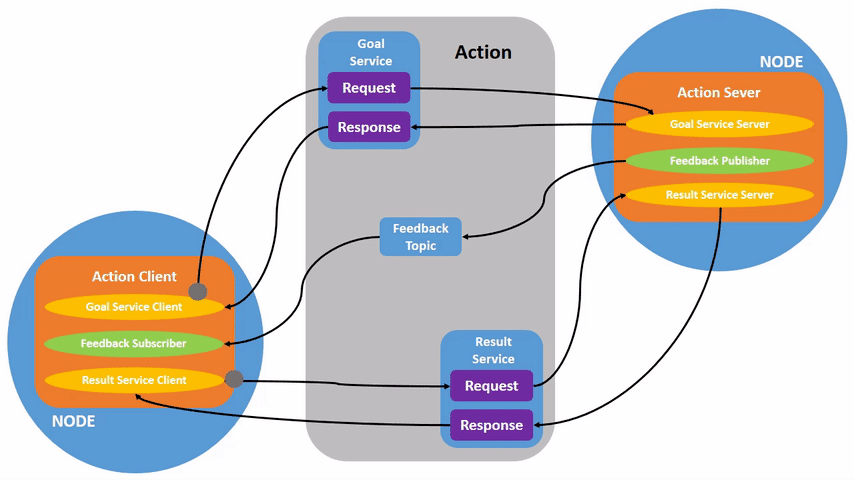
\includegraphics[width=8cm]{img/actionExplanation.png}
		\caption{Vizualizácia akcie v~ROSe~\cite{RosDoc}}
		\label{fig:action}
	\end{figure}

\subsubsection{Parametre}
\label{sec:parametre}

\textbf{Parametre} sú~spôsob, ako môže komunikovať užívateľ so~základnými nastaveniami uzlov
bez~potreby zmenenia kódu a~jeho následnej kompilácie, čo pri~väčších projektoch môže zabrať
aj~trištvrte hodiny. Konfigurácie sa definujú v~\textit{yaml} konfiguračnom súbore. V~ňom si
môžeme zadefinovať mená jednotlivých parametrov a~ich základné hodnoty. Tie si programátor
vie v~programe vytiahnuť pomocou API, \acrlong{API}, (Aplikačné Programovacie Rozhranie) v~ROSe.

\subsection{ROS1}
\label{subsec:ros1}

ROS bol prvýkrát vydaný v~roku 2007. Jeho tvorcovia \textit{Keenan Wyrobek} and \textit{Eric Berger} zo Stanford
univerzity zacali ROS ako osobny projekt za ucelom odstranenia procesu znovuobjavovania kolesa~\cite{rosHistory}.
Ide o~softvér, ktorý sa začal vyvíjať so~zámerom zjednodušiť a~zjednotiť programovanie a~ovládanie robotov.
Od~doby, kedy vznikol prešiel mnohými verziami a~úpravami. Jeho neoddeliteľnou súčasťou sú~štrukturovanie programu
do~uzlov (nodov), komunikácia medzi uzlami, podpora viacerých programovacích jazykov ako sú~C, C++ alebo Python
a~vytváranie balíčkov dostupných širokej verejnosti.

Štrukturalizovanie základov ROS1 je spravené monoliticky. Tvorcovia pritom dbali na~to, aby tento
systém vytvorili čo najstabilnejším spôsobom. Na~počiatku musí byť spustený hlavný program (roscore),
ktorý zabezpečuje vytváranie jednotlivých uzlov. Komunikácia medzi uzlami je zabezpečená prostredníctvom
prepojenia uzlov cez~LAN/WLAN alebo IPC komunikáciu. Ak~sú~uzly spustené na~iných zariadeniach,
tak~sa využíva len komunikácia cez~sieť. Roscore ďalej poskytuje parametre jednotlivým uzlom
z~parametrového servera. Jeho najdôležitejšou úlohou je zabezpečenie komunikácie uzlov v~programe.

\clearpage

Aj~napriek mnohým výhodám má ROS1 nedostatky, ktoré sa ťahajú už~od~jeho počiatkov. Sú~to~napríklad:

\begin{itemize}
	\item Nepostačujúca distribuovanosť systému. Všetky uzly sa spoliehajú na~funkčnosť roscore-u,
	\item ROS1 je písaný v~starom štandarde, to~vnáša do~programu technologický dlh a~bezpečnostné riziká,
	\item Kvalita komunikácie sa nedá ovplyvniť,
	\item Preddefinované vláknové moduly~\cite{ROS2design},
	\item Možnosť užívateľa predefinovať základne prvky ROS-u.
\end{itemize}

Kvôli takýmto problémom a~nedostatkom sa začala vyvíjať nová verzia ROSu, ROS2. Tá mala vyriešiť tieto problémy a~zlepšiť funkcionalitu
prvej verzie. V~roku 2025 sa skončí podpora poslednej distribúcie ROS1 menom \textit{Noetic}. Preto~je odporúčané začínať nové projekty
v~ROS2.

\subsection{ROS2}
\label{subsec:ros2}

\begin{figure}[!htbp]
	\centering
	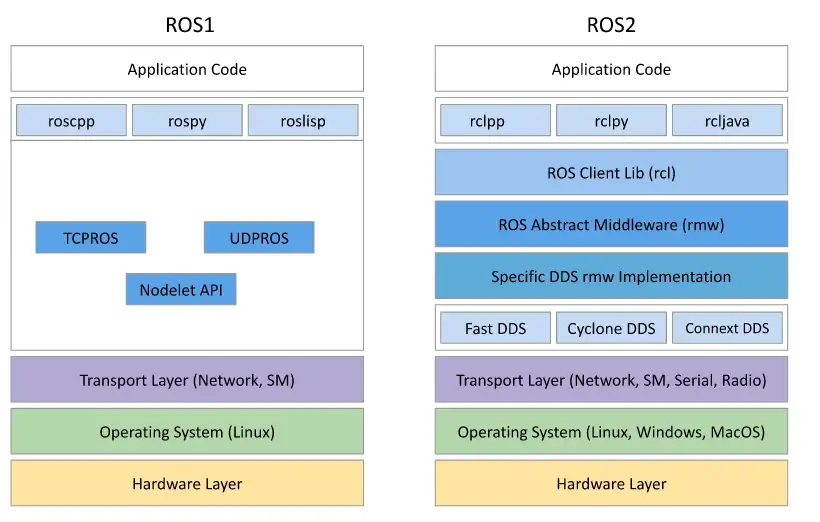
\includegraphics[width=15cm]{img/strukturaRos1Ros2.png}
	\caption{Porovnanie štruktúr ROS1 a~ROS2~\cite{comparison}}
	\label{fig:struktury}
\end{figure}

Ako už~bolo spomenuté zámerom vývoja ROS2 bolo zlepšenie funkcionality a~bezpečnosti systému. Jeden z~dôsledkov tohto vývoja je, že~ROS2
nie je spätne kompatibilný software. Podstata toho, ako sú~zoskupované uzly a~ako spolu komunikujú je diametrálne odlišná od~ROS1. Z~tohto dôvodu
bol vyvinutý takzvaný rosbridge, ktorý zabezpečuje kompatibilitu medzi verziami. Nie je to~ale~trvalé riešenie. Odporúčané je nástroj
využívať a~počas toho prepisovať kód z~verzie 1 do~verzie 2. Komunikácia prebieha v~ROS2 rovnakým spôsobom ako v~ROS1. Pomocou tém
\ref{sec:topic}, služieb \ref{sec:services} a~akcií \ref{sec:actions}.

Táto podobnosť končí na~najvyššej vrstve. Ako sme videli na~Obr.~\ref{fig:struktury}. Štruktúra ROS2 je rozdelená do~viacerých vrstiev.
Najdôležitejšie je pre~nás vedieť, že~komunikácia je spracovávaná modelom DDS (Služba distribúcie údajov) z~anglického
(\acrlong{DDS}). DDS obsahuje podobne dizajnov vzory ale poskytuje väčšiu ovládateľnosť komunikácie systémov, zatiaľ
čo odstraňuje všetky vrstvy, ktoré zabraňujú debugovaniu~\cite{ElectronicDesign}. Tento model zároveň zlepšuje výkon,
stabilitu a~bezpečnosť modelu oproti ROS1. Je založený na~TCP/IP a~UDP/IP protokole. Z~obrázku Obr.~\ref{fig:struktury}
vyčítame aj~lepšie rozloženie modulov. To~zabezpečuje jednoduchšie prispôsobovanie systému pre~nové funkcionality. Podpora operačných systémov
sa v~ROS2 rozšírila aj~o~Windows, Mac OS či~RTOS (Operačné systémy reálneho času) z~anglického \acrlong{RTOS}. Operačné systémy nie sú~jediné
rozšírenie ohľadom kompatibility. S~ROS2 je možné programovať už~aj~v~Jave či~Matlabe. Tvorcovia mysleli aj~na~programátorov a~pridali rozšírené
možnosti testovania, debugovania či~nasadzovania programu do~reálneho využitia.

Testovanie prebieha pomocou použitia Google testov. Debugovanie je možné uskutočniť pomocou debuggera gnu-gdb. Pri~spustení programu
cez~spúšťací súbor (launch file) je potrebné pridať príkaz na~spustenie spomenutého debugovacieho programu.

ROS2 má necentralizovanú štruktúru, a~preto~pri~spúšťaní programov už~nie je potrebné mať spustený roscore. Ak~teda spadne jeden uzol všetky
ostatné uzly budú fungovať naďalej. V~ROS1 sme vedeli ovplyvniť počet uchovaných správ komunikácie pokým nepretiekol zásobník, ktorý ich uchovával
na~neskoršie použitie. V~ROS2 vieme implementovať túto schopnosť použitím takzvanej \textit{QoS} triedy (kvalita komunikácie), z~anglického \acrlong{QoS}.
Pomocou tejto triedy vieme aj~zmeniť kvalitu komunikácie. Vieme si zadefinovať, či~by sme radšej stratili niektoré správy, ale~dostali by~sme
všetky rýchlo. Alebo aby sa zabezpečilo, že~dostaneme všetky správy, ktoré boli vyslané, aj~keby to~trvalo dlhšie. Dokonca si vieme zadefinovať
maximálny čas, ktorý budeme čakať na~ďalšiu správu.

Ak~by bol užívateľ veľmi schopný programátor a~potreboval by si zmeniť triedy, ktoré definujú základnú funkcionalitu ROS-u, tak~aj~toto je možné.
Jednou z~takýchto funkcionalít je, že~užívateľ si vie predefinovať triedu, ktorá bude alokovať miesto na~(IPC) komunikáciu (medziprocesovú komunikáciu).
K~tomuto bodu je dodať, že~tento prípad je špecifický a~väčšina programátorov sa s~takouto možnosťou do~kontaktu nedostane.

Pri~všetkých týchto zlepšeniach nemôžeme zabudnúť spomenúť aj~nasledovný nedostatok. Keďže ROS2 je mladší ako ROS1 nájdeme k~nemu menej dokumentácie.
Pridaním veľkého počtu funkcionalít začal vznikať problém pre~začiatočníkov s~porozumením niektorých kódov. Avšak tento problém je nedostatkom,
ktorý časom zanikne. V~čase písania tejto práce pribudli na~stránke dokumentácie minimálne 2 strany popisujúce pokročilejšie Funkcionality druhej
verzie ROSu.

\subsection{Rozdiely}

Čo je určite dobrou správou pre~všetkých programátorov, ktorí robili v~prvej verzii a~sú~zvyknutí na~jej štandardy a~funkcionalitu. Tak~títo
sa nemajú čoho obávať. Prechod z~ROS1 na~ROS2 je dosť priamočiary. Čo sa zmenilo je spôsob písania kódu, ale~koncepty ostali všetky rovnaké.
V~tejto sekcii nebudeme písať konkrétne kódy, budeme len opisovať čo je podobné a~čo zasa rozdielne medzi verziami spomínaného systému. Keďže
celý projekt bol písaný v~programovacom jazyku C++ tak~sa aj~tieto zmeny budu týkať hlavne jazyka C++.

\subsubsection{Štandard jazyka}

	Pokým ROS1 bola písaná v~štandarde C++03 tak~ROS2 je už~písaná v~novom štandarde. A~to~hlavne C++11, ale~používa aj~nejaké časti z~C++14
	a~C++17. To~zahŕňa inicializovanie templatov a~ich používanie. Tým, že~ROS2 je stále nová a~stále vyvíjajúca sa platforma, tak~môžeme očakávať aj~časti
	kódu, ktoré budú podporovať najnovší C++ štandard a~to~štandard z~rokov 2020 a~2023.

	Definície a~deklarácie templatov sú~na~knihu samú o~sebe, preto~do~detailov nebudeme zachádzať. Stačí nám vedieť, ako ich inicializovať.
	V~prvej verzii sme definovali všeobecného publishera (publikovateľa) a~definovali sme mu len cez~akú tému má posielať správy. V~druhej verzii
	naväzujeme publishera na~špecifický tip správy akú posielame. Nemôže sa teda stať, že~takýto program by sme skompilovali a~následne, keď
	ho spustíme, tak~by spadol z~dôvodu, že~čítame iný typ správy ako posielame.

\subsubsection{Inicializácia nody (uzla)}

	Tak~isto ako v~prvej verzii aj~v~druhej verzii musíme definovať uzol (node). Rozdiel je v~tom, že~prvá verzia obsahovala NodeHandle (Ovládač uzla)
	a~druhá verzia obsahuje priamo Node (Uzol). V~druhej verzii je zaužívaným štandardom túto nodu predediť a~použiť polymorfizmus pri~objekte,
	ktorý bude existovať počas celej doby vykonávania programu. Pri~prvej verzii tomu tak~nebolo. Tam sme museli vytvoriť už~spomenutý NodeHandle.
	Ten sa nemusel využiť ako base trieda a~nemusel ani~existovať počas celého behu programu.

\subsubsection{Komunikácia}

	DDS (Služba distribúcie údajov) je protokol strednej vrstvy (middleware) implementovaný nad UDP~\cite{ROS2book}. Na~implementáciu tohto protokolu
	je použitý protokol z~IoT (internet veci) (\acrlong{IoT}) sféry. Je to~protokol MQTT. DDS je používaný v~ROS2 na~komunikáciu medzi uzlami. Je
	to~systém správ publikovania (publish) / odoberania (subscribe), ktorý umožňuje uzlom komunikovať medzi sebou bez toho, aby poznali identitu
	ostatných uzlov. Druh komunikácie je v~ROS2 rozšírený ešte o~akcie viď kapitolu~\ref{sec:actions}.

\subsubsection{Parametre}

	ROS1 používa parametrový server, ktorý sa nachádza v~roscore-e. Každý uzol si mohol vytiahnuť parametre, ktoré boli zapísané v~konfiguračnom
	súbore. ROS2 žiadny roscore nemá, preto~sa parametre musia distribuovať iným spôsobom. Parametre v~druhej verzii ROSu patria jednotlivým uzlom.
	To~znamená, že~jednotlivé parametre sa dajú vytiahnuť len daným uzlom. Tieto parametre taktiež existujú len počas existencie daného uzlu. Parametre
	sú~ďalej distribuované pomocou už~spomínaného DDS protokolu. V~prípade, že~sa tieto parametre nepodari vytiahnuť z~konfiguračného súboru. Či už~z~dôvodu,
	že~daný súbor neexistuje, alebo iného dôvodu, tak~sa aplikujú základné hodnoty, ktoré si zvolil užívateľ pri~používaní funkcie na~ich zisťovanie.

\subsubsection{Nodelet alebo komponent}

	ROS1 ponúka možnosť definície uzlov ako uzlík (\texttt{nodelet}). Je to~definovanie uzlu ako zdielanej knižnice (shared library). Je
	to~spôsob ako uľahčiť prácu CPU. Keď sa definuje uzol ako uzlík, tak~jeden proces môže spracovávať programy z~viacerých takýchto uzlíkov.
	Táto funkcionalita sa nachádza aj~v~ROS2. Volá sa komponent (\texttt{component}). Vylepšením oproti nodelet-om je zjednotenie aplikačnej
	implementácie (API). Pokým nodelet-y mali vlastný spôsob implementácie v~ROS1 tak~v~ROS2 je implementácia uzla a~komponentu rovnaká.
	Pri~komponente sa musí len naviac definovať, že~daný komponent existuje pomocou makra. Použitie komponentov zjednodušuje prácu CPU
	a~používa sa hlavne v~zariadeniach, ktoré majú obmedzený výkon výpočtovej techniky. Sú~to~napríklad mikroprocesory, ktoré ovládajú roboty.

\subsubsection{Kompilácia}

	Zmenou verzii sa zmenil aj~spôsob kompilácie programu. ROS1 bol kompilovaný pomocou \texttt{catkin} build systému. Catkin je založený
	na~programe \texttt{cmake}. Jeho nastavenie dependencií je konfigurované pomocou súboru \texttt{package.xml}. ROS2 prešiel na~viac
	nastaviteľný systém \texttt{Colcon}. Tento systém je na~rozdiel od~catkin-u založený na~Python-e a~jeho dependencie sa nastavujú pomocou
	\texttt{setup.py} súboru. V~prípade colcon-u si môžeme definovať spôsob kompilácie to~znamená, že~môžeme nastaviť, ako sa budú spracovávať
	dependencie. Ponúkané možnosti sú~\texttt{catkin\_make}, \texttt{catkin\_make\_isolated}, \texttt{catkin\_tools} a~\texttt{ament\_cmake}.
	Jednou s~najviac používaných možností je \texttt{ament\_cmake}. Je založený na~programe \texttt{cmake} a~spolupracuje so~systémom \texttt{colcon}.
	Z~tohto dôvodu mu vieme definovať dependencie pomocou xml súboru ako tomu bolo v~ROS1 pričom možnosť definície pomocou Python skriptu ostáva.
	Je to~jeden zo~spôsobov, ako zmenšiť rozdiel medzi ROS1 a~ROS2.

\subsubsection{Vlákna}

	ROS1 dovoľuje programátorom vybrať si medzi jedno vláknovým a~viac vláknovým vykonávaním programu. Tvorcovia ROS2 si dali zaležať na~modularite
	aj~tejto oblasti kódu. V~druhej verzii ROS-u si vieme zadefinovať typ vykonávania programu separátne pre~každý uzol a~vieme si tento typ
	zadefinovať aj~sami~\cite{ROS2design}.

\subsection{Ros control}
\label{subsec:roscontrol}

Roc\_control je balik naprogramovany v~prostredi ROS1 aj~ROS2. Tym, ze sme si vybrali ROS2 ako prostredie pre~nase riesenie,
tak~by sme pouzili balik ros2\_control.

